\section{Graph databases}

Relational databases often struggle with efficiently managing and querying complex relationships between data entities. 
In contrast, graph databases are specifically designed to handle such tasks using graph structures, which consist of nodes (entities), edges (relationships), and properties.
Graph databases have index-free adjacency, which means that each node directly references its adjacent nodes. 

They not only connect nodes to other nodes but can also link nodes to properties, making the data structure highly flexible for relationship-focused queries.
Graph databases are ideal fit for scenarios where relationships are central to the analysis:
\begin{itemize}
    \item \textit{High performance on relationship queries}: graph databases are optimized for associative datasets, such as social networks.
    \item \textit{Natural fit for object-oriented models}: they inherently support hierarchical structures like parent-child relationships and object classification.
    \item \textit{Efficient traversal}: because nodes directly point to adjacent nodes, queries that involve traversing relationships are much faster compared to relational databases.
\end{itemize}
\renewcommand*{\arraystretch}{2}
\begin{table}[H]
    \centering
    \begin{tabular}{|c|l|}
    \hline
    \multirow{2}{*}{\textbf{Advantages}}    & Easy to extend                                 \\
                                            & Easy to change                                 \\ \hline
    \multirow{2}{*}{\textbf{Disadvantages}} & Complexity growing with the number of elements \\
                                            & Difficult query optimization                   \\ \hline
    \end{tabular}
\end{table}
\renewcommand*{\arraystretch}{2}

\paragraph*{Pattern matching}
Pattern matching is a technique used to find specific structures or relationships within a graph by querying based on patterns of nodes and edges.
This approach allows users to search for complex data relationships by specifying the nodes, types of relationships, and desired properties they want to match.
It is powerful because it enables querying highly interconnected data quickly. 

\subsection{Neo4j}
Neo4j, developed by Neo Technologies, is one of the leading and most popular graph databases available today. 
It is implemented in Java and is open-source, providing a robust platform for managing and querying graph data.
\begin{table}[H]
    \centering
    \begin{tabular}{|c|l|}
    \hline
    \textbf{Feature}                 & \multicolumn{1}{c|}{\textbf{Description}}                                     \\ \hline
    \textit{Schema-free}             & Flexible data model that does not require a predefined schema                  \\ \hline
    \textit{ACID compliant}          & Ensures atomicity, consistency, isolation, and durability                      \\ \hline
    \textit{User-friendly}           & Easy to learn, set up, and use, even for new developers                        \\ \hline
    \textit{Extensive documentation} & Supported by a large, active developer community                                 \\ \hline
    \textit{Multi-language support}  & Compatible with Java, Python, Perl, Scala, and Cypher           \\ \hline
    \end{tabular}
\end{table}
Neo4j is primarily designed as an operational database rather than a dedicated analytics platform. 
It excels at managing relationships and provides efficient access to nodes and connections. 
However, it may be less suited for large-scale, full-graph analyses compared to specialized analytics engines.

\subsubsection{Architecture}
Neo4j's architecture consists of three primary layers:
\begin{itemize}
    \item \textit{Memory Layer}: stores records of nodes, relationships, types, and properties. 
        Nodes and edges are managed separately, streamlining queries that target only specific elements. 
        Neo4j attempts to load as much of the graph into RAM as possible to enable fast data access and analysis.
    \item \textit{Operating System layer}: provides a cache to map elements in RAM to their counterparts in secondary storage, facilitating efficient memory management.
    \item \textit{Execution environment}: as Neo4j is written in Java, it runs on the Java Virtual Machine, which also hosts APIs that allow users to interact with the database.
\end{itemize}
\begin{figure}[H]
    \centering
    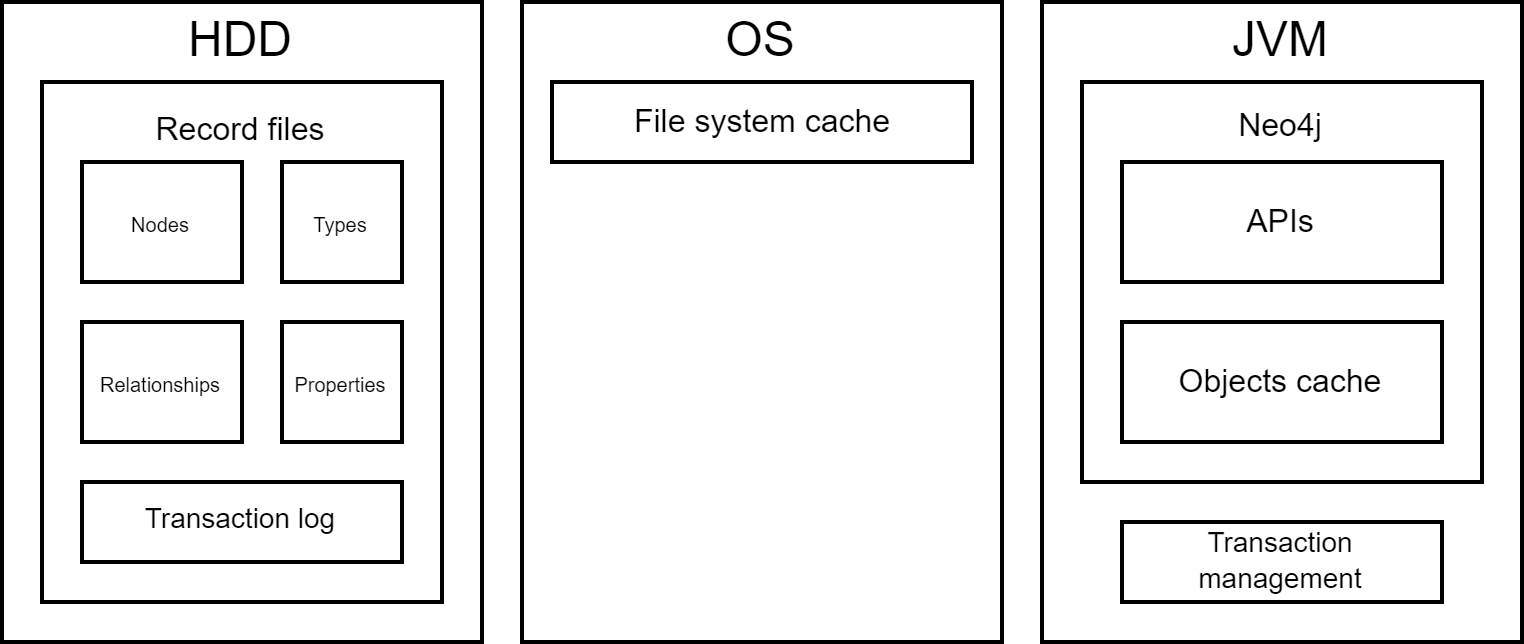
\includegraphics[width=0.65\linewidth]{images/neo4j.png}
    \caption{Neo4j architecture}
\end{figure}
Neo4j uses a declarative query language, Cypher. 
Each query is translated into an execution plan by the query optimizer, which then sends it to the query engine to execute and return results. 
For repeated queries with varying parameters, it's recommended to use parameterized queries to avoid redundant optimization for each execution.

\subsubsection{Data Model}
The Neo4j data model is based on three primary components:
\begin{itemize}
    \item \textit{Nodes}: represent entities, each labeled by types and equipped with attributes (properties).
    \item \textit{Relationships}: define connections between nodes, providing context and capturing relationships between entities.
    \item \textit{Indexes}: improve query performance by allowing fast lookups of nodes and relationships based on properties.
\end{itemize}
\begin{figure}[H]
    \centering
    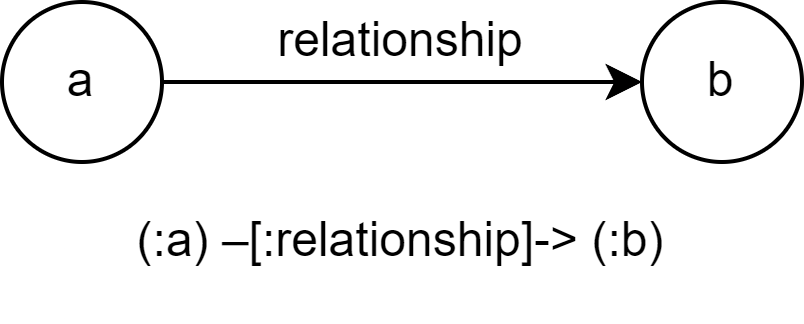
\includegraphics[width=0.50\linewidth]{images/neo4j1.png}
    \caption{Neo4j data model}
\end{figure}

\subsubsection{Query language}
Cypher is the dedicated query language for Neo4j, designed to be both user-friendly and powerful. 
Its declarative nature allows users to specify what data they want to retrieve without needing to define how to obtain it, making query formulation straightforward.

\paragraph*{Data creation and deletion}
Witch Cypher we can create a new node in the following way: 
\begin{lstlisting}[style=Cypher]
CREATE (node:Label {property: value, ... })
\end{lstlisting}
In the same way, we can create relationships between existing nodes: 
\begin{lstlisting}[style=Cypher]
CREATE (n1)-[r:RelationshipType {property: value, ...}]->(n2)
CREATE (n1)-[r:RelationshipType {property: value, ...}]-(n2)
\end{lstlisting}
Remeber that each node may have multiple labels to specify for example a group and a sub-group. 
We may also delete some nodes with all the relationships: 
\begin{lstlisting}[style=Cypher]
MATCH (node:Label {property: value, ... }) 
DETACH DELETE node
\end{lstlisting}
In this query the \texttt{delete} clause allows the removal of nodes and relationships, while the \texttt{detach} removes all the relationships before removing the nodes.
This can also be applied to single relationships: 
\begin{lstlisting}[style=Cypher]
MATCH (n1)-[r:RelationshipType {property: value, ...}]->(n2)
DELETE r
\end{lstlisting}

\paragraph*{Data importing}
Neo4j allows importing an entire graph from a csv file using the Cypher query language:
\begin{lstlisting}[style=Cypher]
USING PERIODIC COMMIT 
LOAD CSV WITH HEADERS FROM "file:data.csv" AS row
CREATE (:Label {property: row.Column1, ... })
\end{lstlisting}
The periodic commit is essential for handling large datasets efficiently, as it commits data in batches to ensure ACID compliance, preventing memory overload and maintaining transaction integrity.

\paragraph*{Data merging}
To avoid creating duplicate nodes or relationships, use the merge operation:
\begin{lstlisting}[style=Cypher]
MERGE (n:Label {property: 'value'})
ON CREATE 
    SET n.property1 = 'new_value'
ON MATCH 
    SET n.lastUpdated = date()
\end{lstlisting}
The merge clause checks if a node with the specified properties exists; if not, it creates it. 
The clause \texttt{on create} is used to set properties when the node is newly created, and \texttt{on match} allows updating properties if the node already exists. 
This approach can also be applied to relationships, ensuring no duplicate edges.

\paragraph*{Indices and constraints}
To improve query performance, create an index on a specific property of a node label:

\begin{lstlisting}[style=Cypher]
CREATE INDEX ON :Label(property)
\end{lstlisting}
This command creates an index on the specified property for nodes with the given label, speeding up searches on that property.
To enforce data integrity, create a constraint on a specific property:

\begin{lstlisting}[style=Cypher]
CREATE CONSTRAINT ON (n:Label)
ASSERT n.property IS UNIQUE
\end{lstlisting}
This command enforces uniqueness on the specified property for nodes with the given label, ensuring no duplicate values for that property across nodes.

\paragraph*{Data querying}
The general structure of a Cypher query is as follows:

\begin{lstlisting}[style=Cypher]
MATCH (n1)-[:RelationshipType]-(n2)
WITH n1, count(n2) AS relationCount
ORDER BY relationCount DESC
SKIP 1 
LIMIT 3
RETURN DISTINCT n1
\end{lstlisting}
In this query:
\begin{itemize}
    \item Aggregation functions like \texttt{count} can be utilized to calculate values.
    \item The \texttt{with} clause explicitly separates parts of the query and declares variables for subsequent sections.
    \item \texttt{skip} is used to bypass a specified number of results, while \texttt{limit} restricts the total number of results returned.
    \item \texttt{distinct} is used to return all different elements.
\end{itemize}
Additionally, appending an asterisk (\texttt{*}) to a relationship allows for retrieving all nodes that are not directly connected by that relationship type.

\begin{table}[H]
    \centering
    \begin{tabular}{|c|l|}
    \hline
    \textbf{Cypher pattern}                                & \textbf{Description}                                           \\ \hline
    \texttt{(n:Person)}                                   & Node with the \texttt{Person} label.                                   \\ \hline
    \texttt{(n:Person:Swedish)}                          & Node with both \texttt{Person} and \texttt{Swedish} labels.                     \\ \hline
    \texttt{(n:Person\string{name:\$value\string})}                & Node with the given properties.                             \\ \hline
    \texttt{()-[r\string{name:\$value\string}]-()}                 & Matches relationships with the given properties.            \\ \hline
    \texttt{(n)-->(m)}                                   & Relationship from \texttt{n} to \texttt{m}.                                     \\ \hline
    \texttt{(n)--(m)}                                    & Relationship in any direction between \texttt{n} and \texttt{m}.                \\ \hline
    \texttt{(n:Person)-->(m)}                            & Node \texttt{n} labeled \texttt{Person} with a relationship to \texttt{m}.              \\ \hline
    \texttt{(m)<-[:Know]-(n)}                           & \texttt{Know} relationship from \texttt{n} to \texttt{m}.                               \\ \hline
    \texttt{(n)-[:Know|:Love]->(m)}                    & \texttt{Know} or \texttt{Love} relationship from \texttt{n} to \texttt{m}.                      \\ \hline
    \texttt{(n)-[r]->(m)}                                & Binds relationship to \texttt{r}.                                      \\ \hline
    \texttt{(n)-[*1..5]->(m)}                            & Variable length path (1 to 5) from \texttt{n} to \texttt{m}.                   \\ \hline
    \texttt{(n)-[*]->(m)}                                & Variable length path from \texttt{n} to \texttt{m}.                             \\ \hline
    \texttt{(n)-[:Know]->(m\string{property:\$value\string})}    & \texttt{Know} relationship from \texttt{n} to \texttt{m} with a property.               \\ \hline
    \end{tabular}
\end{table}

\paragraph*{Finding paths}
In Cypher, there are several functions available to identify paths within the graph between nodes. 
These functions allow you to efficiently navigate relationships and retrieve relevant data.
To find the shortest paths between nodes, you can use the following Cypher queries:
\begin{itemize}
    \item \textit{Single shortest path}: this function retrieves a single shortest path between two nodes and the path can traverse up to six relationships: 
        \begin{lstlisting}[style=Cypher]
shortestPath((n1:Label)-[*..6]-(n2:Label))
        \end{lstlisting}
    \item \textit{All shortest paths}: if you want to find all possible shortest paths between two nodes, use this query. 
        It ensures that every shortest path is considered: 
        \begin{lstlisting}[style=Cypher]
allShortestPaths((n1:Label)-[*..6]->(n2:Label))
        \end{lstlisting}
\end{itemize}
To count the number of paths that match a specific pattern, you can use the following query. 
This example counts paths with a given structure originating from node \texttt{n} and extending through two relationships:
\begin{lstlisting}[style=Cypher]
size((n)-->()-->())
\end{lstlisting}